\documentclass[12pt,aspectratio=169]{beamer}

\usepackage[spanish,es-noshorthands]{babel}
\usepackage[utf8]{inputenc}
\usepackage{amsmath,amssymb}
\usepackage[numbers]{natbib}
\usepackage{booktabs}
\usepackage{textcomp}

\usetheme{Madrid}
\usecolortheme{whale}
\setbeamertemplate{navigation symbols}{}
\setbeamertemplate{caption}[numbered]
\setbeamertemplate{footline}[frame number]
\setbeamercovered{transparent}

\title[ngVLA: mapas sintéticos de SFR a alto $z$]{Producción de observaciones sintéticas del ngVLA\\ de galaxias a alto corrimiento al rojo}
\subtitle{Avance de práctica final}
\author{Lobsang Derek Méndez Ojeda}
\institute[USAC]{
    Escuela de Ciencias Físicas y Matemáticas\\
    Universidad de San Carlos de Guatemala\\[4pt]
    \small Asesor externo: Dr.\ Eric F.\ Jiménez-Andrade (IRyA-UNAM)\\
    \small Asesor local: Dr.\ Rodrigo Sacahuí (ECFM-USAC)
}
\date{\today}

\begin{document}

% ---------------------------------------------------------------
\begin{frame}
    \titlepage
\end{frame}

\begin{frame}{Contenido}
    \tableofcontents
\end{frame}

% =================================================================
\section{Contexto y motivación}
% =================================================================

\begin{frame}{Interferometría: el compromiso resolución--sensibilidad}
    \begin{itemize}
        \item Un plato único está limitado por difracción a
        $\theta \sim \lambda/D$: resolver formación estelar a alto $z$
        (fracciones de arcosegundo) exige líneas de base de km.
        \item Un interferómetro mide visibilidades en el plano $uv$
        \citep{tms2017,condon2016}; su distribución fija dos propiedades
        en tensión directa:
        \begin{itemize}
            \item \textbf{Resolución angular} $\uparrow$ con la línea de
            base máxima (config.\ A, extendida).
            \item \textbf{Sensibilidad al brillo superficial extendido}
            $\uparrow$ con líneas de base cortas (config.\ B, compacta).
        \end{itemize}
        \item Además, a $D$ fija: $\theta\sim\lambda/D$ empeora la
        resolución al bajar en frecuencia -- mismo compromiso, ahora entre
        \emph{banda observada} y resolución.
    \end{itemize}
    \vfill
    \small Este proyecto reproduce ambos efectos (beam + ruido
    correlacionado) para estimar si SINGS proyectada a $z>1$ es
    detectable y resoluble con cada instrumento.
\end{frame}

\begin{frame}{El ngVLA}
    \begin{columns}[T]
        \begin{column}{0.52\textwidth}
            \begin{itemize}
                \item 263 antenas (244$\times$18\,m + 19$\times$6\,m),
                Nuevo México -- México -- Canadá.
                \item Rango de frecuencia: \textbf{1.2--116 GHz}.
                \item Resolución: mas hasta $\mu$as; sensibilidad
                $>10\times$ el VLA actual.
                \item Puente entre ALMA ($>100$ GHz) y el futuro SKA
                ($<1$ GHz).
                \item 5 objetivos científicos clave, incluyendo mapear la
                evolución galáctica a lo largo del tiempo cósmico
                \citep{ngvla}.
            \end{itemize}
        \end{column}
        \begin{column}{0.44\textwidth}
            \centering
            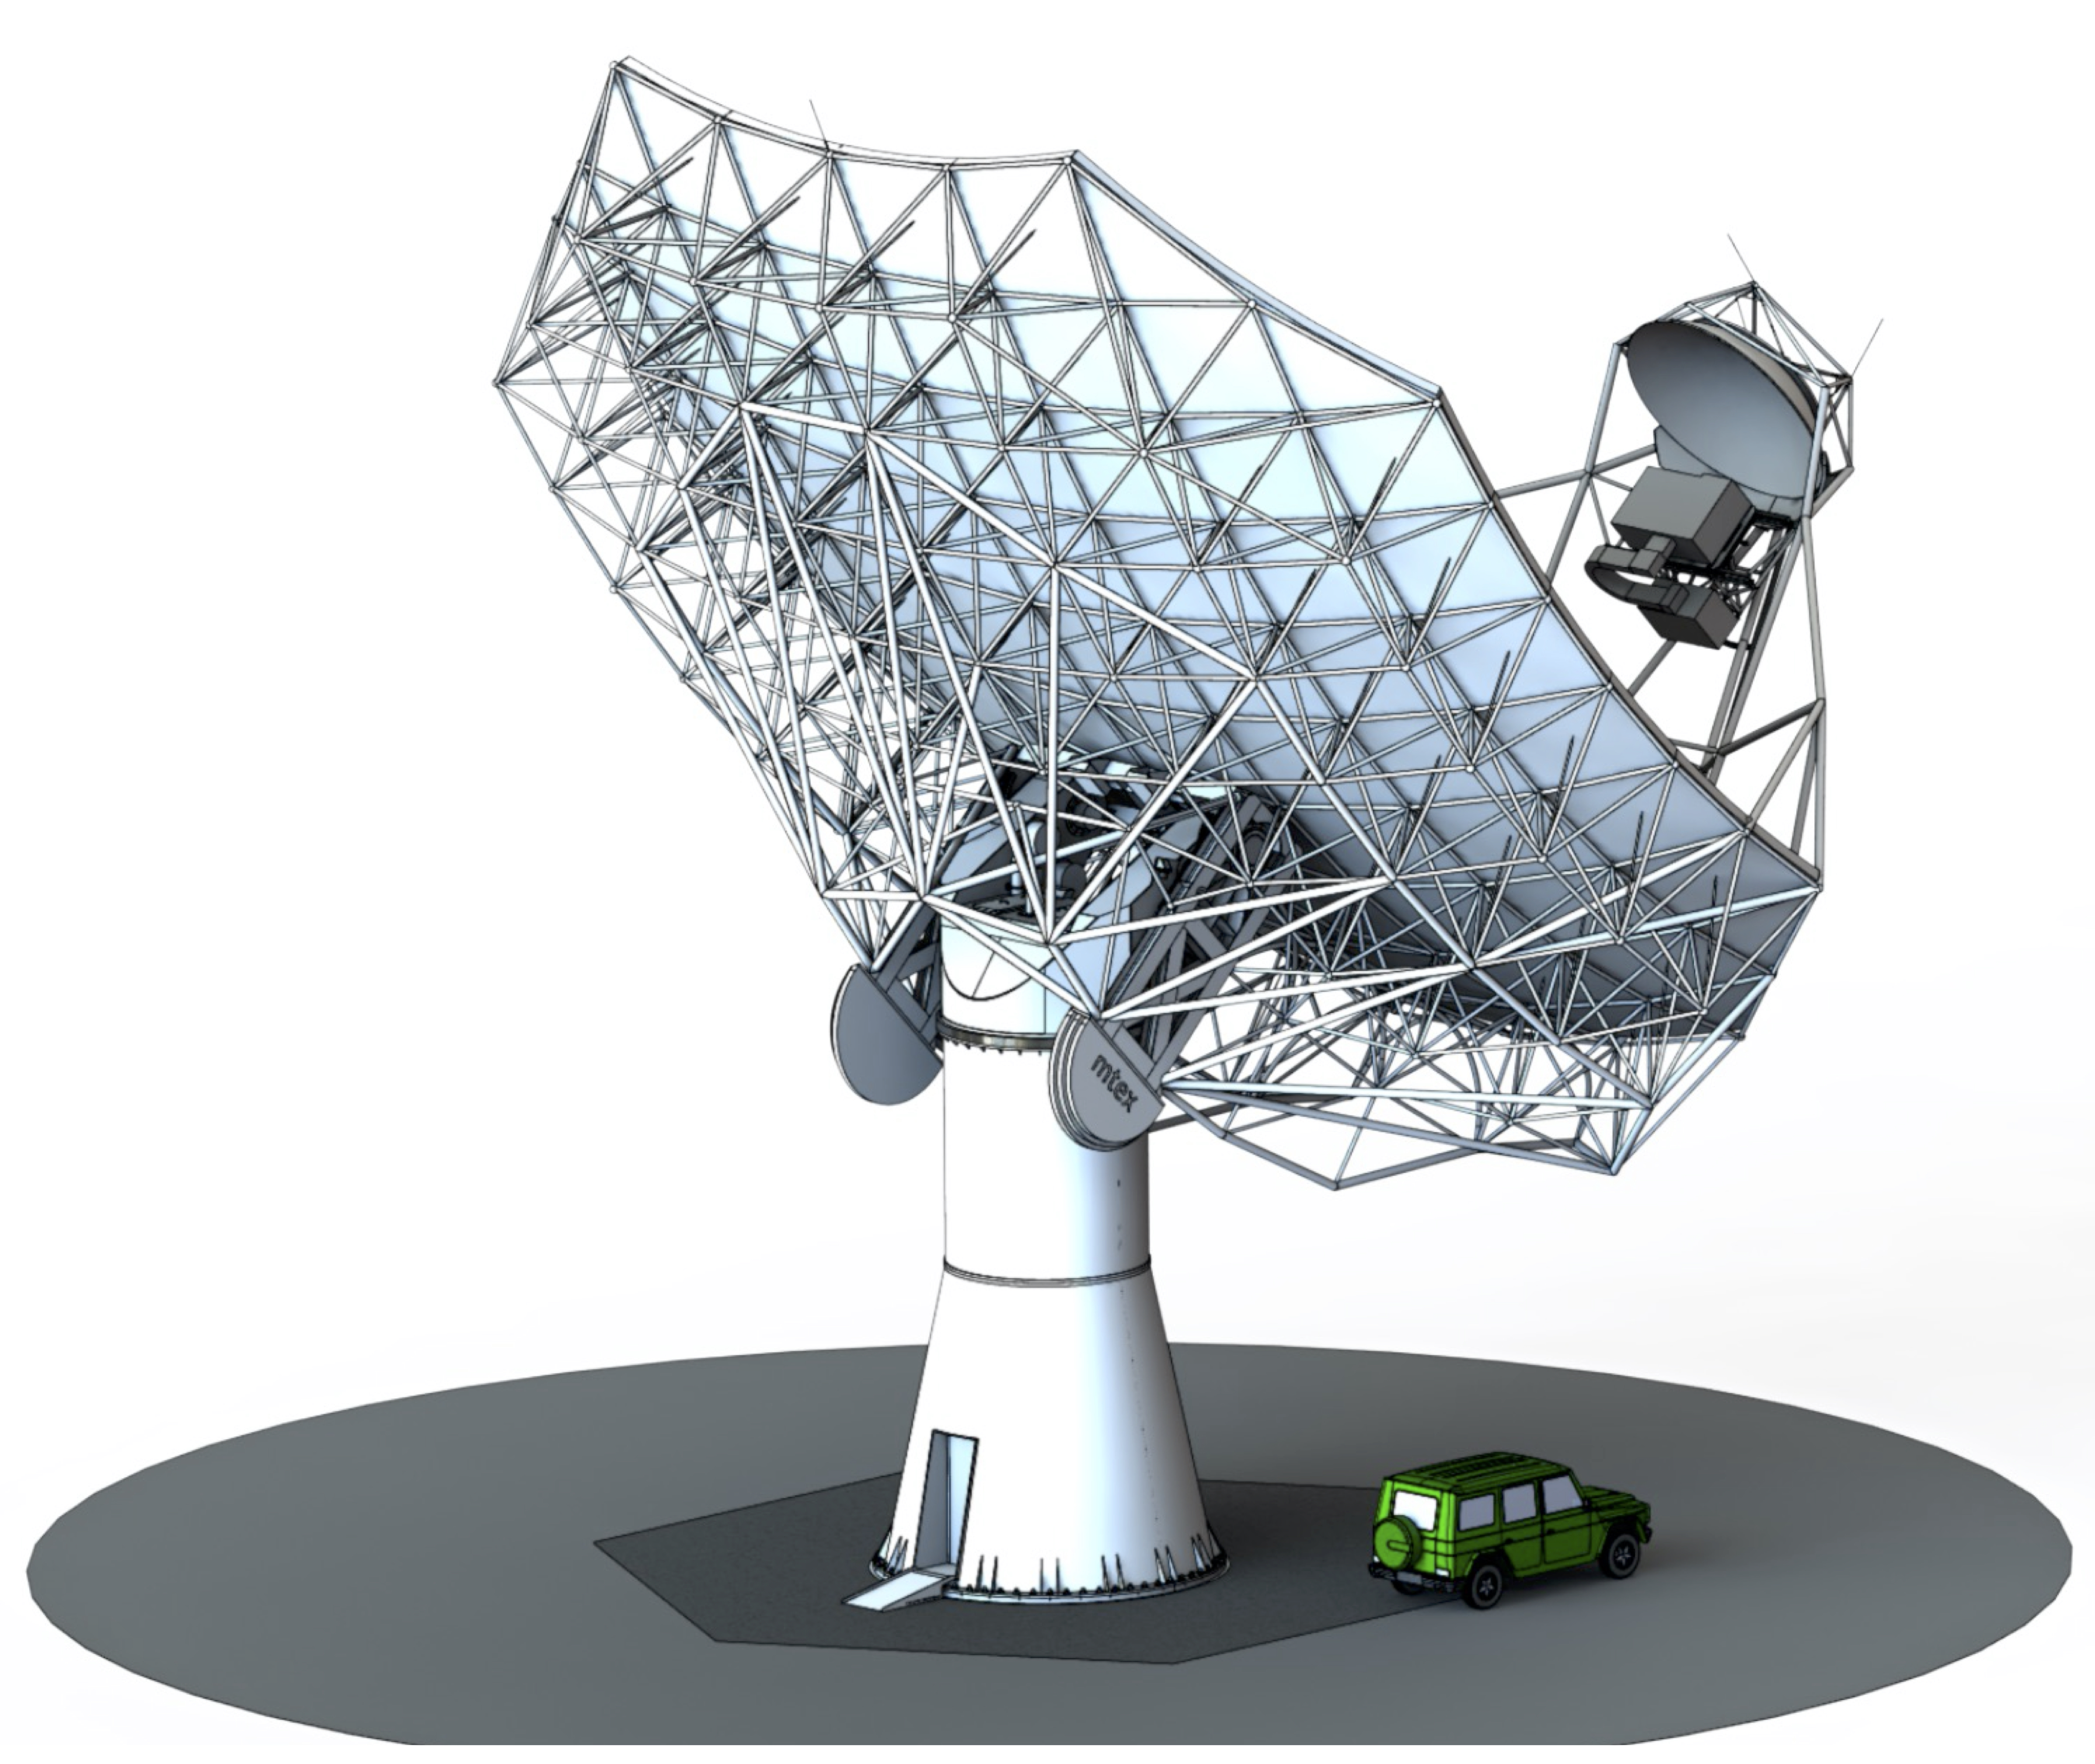
\includegraphics[width=\linewidth]{images/ngVLA.jpg}\\
            \tiny NRAO/ngVLA
        \end{column}
    \end{columns}
\end{frame}

\begin{frame}{Radio continuo como trazador de SFR}
    \begin{itemize}
        \item A frecuencias $\sim$GHz, la emisión de radio continuo de
        una galaxia formadora de estrellas combina:
        \begin{itemize}
            \item \textbf{Sincrotrón} (domina): electrones relativistas en
            remanentes de SN ($M\gtrsim8\,M_\odot$) $\Rightarrow$ traza
            SFR en escalas $\sim$decenas de Myr.
            \item \textbf{Libre-libre}: gas ionizado en regiones HII
            $\Rightarrow$ traza SFR casi instantánea.
        \end{itemize}
        \item Espectro sincrotrón: $S_\nu \propto \nu^{-\alpha}$,
        $\alpha\approx0.7$--$0.8$.
        \item \textbf{Ventaja central}: el polvo no absorbe ni dispersa
        radio $\Rightarrow$ SFR sin corrección por extinción, crítico para
        galaxias polvorientas y de alto $z$.
        \item Corrección-$K$ cosmológica: $\nu_{\mathrm{obs}} =
        \nu_{\mathrm{em}}/(1+z)$ -- un instrumento a frecuencia fija
        muestrea, en el marco de la galaxia, una frecuencia creciente
        con $z$.
    \end{itemize}
\end{frame}

\begin{frame}{Secuencia principal y el modelo de Leslie et al.\ (2020)}
    \begin{columns}[T]
        \begin{column}{0.5\textwidth}
            \begin{itemize}
                \item SFR vs.\ $M_*$: bimodal -- secuencia principal
                (formadoras activas) vs.\ galaxias \emph{quenched}
                \citep{noeske2007,whitaker2012}.
                \item VLA-COSMOS 3\,GHz ($>190{,}000$ galaxias):
                parametrización continua SFR$(M_*,z)$ hasta $z\sim5$
                \citep{leslie2020}.
                \item sSFR crece fuertemente con $z$: máximo de densidad
                cósmica de SFR en $z\sim1$--$3$, el \emph{cosmic noon}
                \citep{madau2014}.
                \item Motiva proyectar SINGS ($z\approx0$) al régimen de
                formación estelar elevada de esa época.
            \end{itemize}
        \end{column}
        \begin{column}{0.46\textwidth}
            \centering
            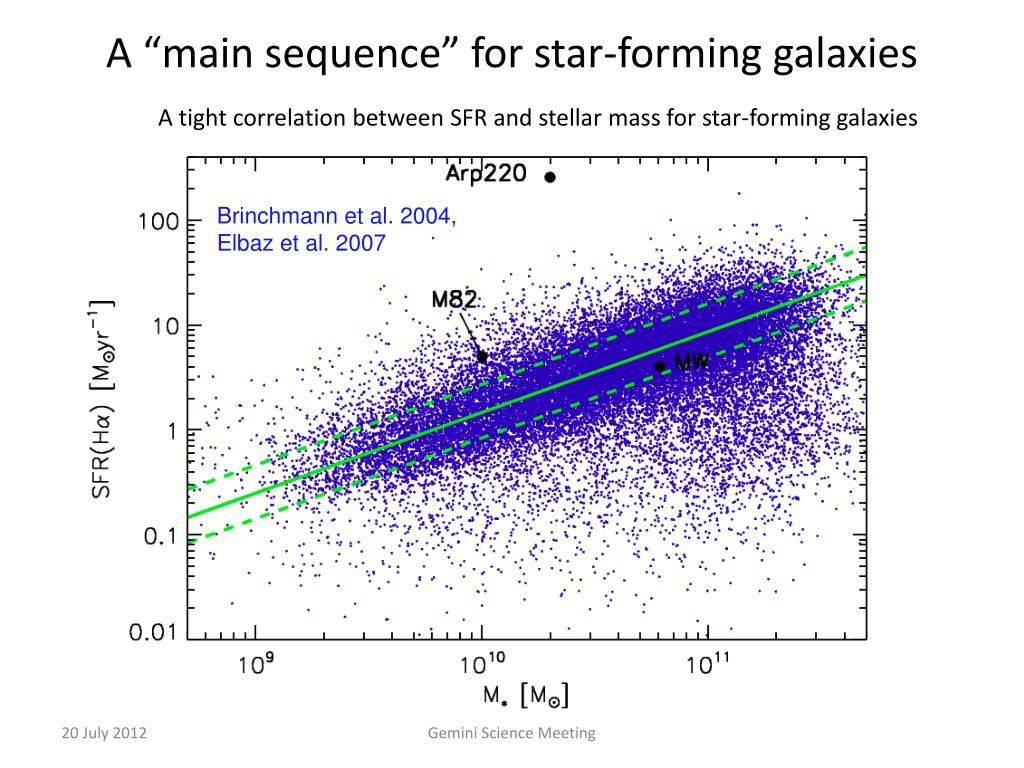
\includegraphics[width=\linewidth]{images/Secuencia_principal_formacion_estelar.jpg}
        \end{column}
    \end{columns}
\end{frame}

% =================================================================
\section{Objetivos}
% =================================================================

\begin{frame}{Objetivo general}
    \begin{block}{}
        Evaluar la capacidad del ngVLA para obtener mapas sintéticos de
        formación estelar en continuo de radio en galaxias a alto
        corrimiento al rojo, comparando su desempeño frente al Jansky VLA
        actual.
    \end{block}
    \begin{block}{Objetivos específicos}
        \begin{enumerate}
            \item Investigar las capacidades técnicas del ngVLA.
            \item Generar mapas de entrada a partir de SINGS, reescalados
            en SFR y proyectados a distintos $z$.
            \item Simular la respuesta instrumental (beam + ruido) del
            ngVLA y del VLA.
            \item Comparar resolución y sensibilidad entre ambos
            instrumentos, a beams equivalentes.
            \item Documentar y presentar los resultados.
        \end{enumerate}
    \end{block}
\end{frame}

% =================================================================
\section{Metodología}
% =================================================================

\begin{frame}{Pipeline: visión general}
    \begin{center}
    \begin{tabular}{c}
    Imagen H$\alpha$ SINGS (continuo restado) \\
    $\big\downarrow$ normalizar a SFR objetivo ($I^+=\max(I,0)$) \\
    Mapa de SFR [$M_\odot\,\mathrm{yr^{-1}}$] \\
    $\big\downarrow$ $L_\nu = \mathrm{SFR}/C$ \\
    Mapa de luminosidad de radio [erg\,s$^{-1}$\,Hz$^{-1}$] \\
    $\big\downarrow$ $D_L(z)$, corrección-$K$ \\
    Mapa de flujo observado a $z$ [Jy] + WCS \\
    $\big\downarrow$ CASA: \texttt{importfits} $\to$ \texttt{imsmooth} $\to$ \texttt{exportfits} \\
    $\big\downarrow$ + ruido correlacionado (rms nominal ngECT/ECT) \\
    \textbf{Mapa simulado ngVLA/VLA a $z$}
    \end{tabular}
    \end{center}
    \vfill
    \small 14 galaxias SINGS con H$\alpha$ disponible $\times$ 5 $z$
    $\times$ 4 configuraciones instrumentales.
\end{frame}

\begin{frame}{Redshifts simulados: cobertura de la historia cósmica}
    \begin{center}
    \begin{tabular}{ccc}
    \toprule
    $z$ & SFR ($M_\odot\,\mathrm{yr^{-1}}$) & Edad del Universo (Gyr) \\
    \midrule
    0.4 & 1.5  & 9.18 \\
    1.0 & 7    & 5.75 \\
    2.0 & 40   & 3.22 \\
    3.0 & 100  & 2.11 \\
    5.0 & 300  & 1.15 \\
    \bottomrule
    \end{tabular}
    \end{center}
    \begin{itemize}
        \item SFR objetivo: secuencia principal de \citet{leslie2020} a
        $M_*=10^{10.5}\,M_\odot$ (masa característica $M^*$ de la función
        de masa estelar local).
        \item $\Lambda$CDM plano: $H_0=70$, $\Omega_M=0.3$,
        $\Omega_\Lambda=0.7$ (\texttt{astropy.cosmology}).
        \item No arbitrarios: cubren $\sim$91\% de la historia cósmica
        transcurrida (de 68\% a 9\% de la edad actual del Universo).
    \end{itemize}
\end{frame}

\begin{frame}{De SFR a flujo observado}
    \begin{equation*}
        L_\nu = \frac{\mathrm{SFR}}{C}\, ,\qquad
        C = 4.87\times10^{-29}\ M_\odot\,\mathrm{yr^{-1}}\,(\mathrm{erg\,s^{-1}\,Hz^{-1}})^{-1}
    \end{equation*}
    \vspace{-4pt}
    consistente con \citet{condon1992,bell2003,murphy2011} (factor
    $\sim$1--2 según IMF/banda de calibración).
    \begin{equation*}
        S_\nu(z) = \frac{L_\nu}{4\pi D_L(z)^2\,(1+z)^{1-\alpha}}
        \left(\frac{\nu_{\mathrm{rest}}}{\nu_{\mathrm{obs}}}\right)^{-\alpha}
    \end{equation*}
    \begin{itemize}
        \item $D_L(z)$: distancia de luminosidad, \texttt{FlatLambdaCDM}.
        \item $(1+z)^{1-\alpha}$: corrección-$K$ cosmológica.
        \item $(\nu_{\mathrm{rest}}/\nu_{\mathrm{obs}})^{-\alpha}$:
        extrapolación espectral entre la calibración (1.4 GHz) y la
        frecuencia efectivamente observada.
        \item Escala espacial física asignada vía kpc/arcsec$(z)$ +
        encabezado WCS completo $\Rightarrow$ tratable como observación
        real en CASA.
    \end{itemize}
\end{frame}

\begin{frame}{Configuraciones instrumentales: el VLA como referencia}
    \begin{itemize}
        \item El VLA aporta dos resoluciones nativas reales (config.\ A y
        B). El ngVLA \textbf{no} tiene configuraciones discretas: se usó
        siempre el \emph{Main array} completo.
        \item ``ngVLA-A/B'' es una \textbf{etiqueta interna}: ¿qué ruido
        rms alcanza el Main array del ngVLA a las mismas resoluciones que
        ofrece el VLA de forma nativa? $\Rightarrow$ aísla sensibilidad de
        resolución angular.
        \item Beam y ruido \textbf{no calculados analíticamente}: se
        tomaron de las calculadoras de exposición oficiales (ngECT / VLA
        ECT), 20\,h de integración, banda de 10~GHz.
    \end{itemize}
    \begin{center}
    \small
    \begin{tabular}{lccc}
    \toprule
    Config. & Beam & Ruido rms/beam & Fuente \\
    \midrule
    ngVLA -- A & $0.293''$ & $28.44$ nJy & ngECT \\
    ngVLA -- B & $0.961''$ & $32.68$ nJy & ngECT \\
    VLA -- A   & $0.293''$ & $0.56\ \mu$Jy & ECT \\
    VLA -- B   & $0.961''$ & $0.56\ \mu$Jy & ECT \\
    \bottomrule
    \end{tabular}
    \end{center}
\end{frame}

\begin{frame}{Simulación instrumental: convolución + ruido correlacionado}
    \begin{itemize}
        \item \texttt{imsmooth} (CASA): convoluciona con kernel gaussiano
        (beam del instrumento) $\Rightarrow$ conserva \textbf{flujo total},
        no brillo superficial (entrega Jy/píxel).
        \item \textbf{Paso crítico}: reescalar a Jy/beam antes de sumar
        ruido, o la señal queda 3--5 órdenes de magnitud bajo el piso de
        ruido:
        \begin{equation*}
            \Omega_{\mathrm{beam}} = 1.1331\,\theta_{\mathrm{beam}}^2,\quad
            I_{\mathrm{Jy/beam}} = I_{\mathrm{Jy/pix}}\cdot
            \frac{\Omega_{\mathrm{beam}}}{\Omega_{\mathrm{pix}}}
        \end{equation*}
        \item Ruido blanco gaussiano ($\sigma=$ rms nominal), convolucionado
        con kernel FWHM = beam, normalizado en $L^2$ (no $L^1$) para
        preservar $\sigma$ tras la convolución.
        \item Resultado: mapa con pérdida de resolución \emph{y} ruido
        correlacionado espacialmente, listo para evaluar detectabilidad
        realista.
    \end{itemize}
\end{frame}

% =================================================================
\section{Control de calidad}
% =================================================================

\begin{frame}{Tres problemas metodológicos identificados y corregidos}
    \small
    \begin{enumerate}
        \item \textbf{Recorte no centrado en el núcleo}: la normalización
        de SFR se hacía sobre el fotograma H$\alpha$ completo, sin
        recortar antes $\Rightarrow$ artefactos fuera del disco competían
        por el presupuesto de SFR (25--55\% del flujo fuera del disco real
        en 10/14 galaxias). \textbf{Fix}: recorte centrado en
        \texttt{OBJCTX}/\texttt{OBJCTY} \emph{antes} de normalizar.
        \item \textbf{Inversión de signo} (ngc4254: 97.4\% píxeles
        negativos; ngc4321: 68.9\%): suma total negativa $\Rightarrow$
        factor de escala negativo $\Rightarrow$ mapa de SFR invertido.
        \textbf{Fix}: normalizar solo sobre $I^+=\max(I,0)$.
        \item \textbf{Estrellas de campo mal sustraídas} (ngc3627,
        ngc4594, ngc5055): fuente compacta espuria separada del núcleo.
        \textbf{Fix}: máscara circular manual por galaxia (no filtro
        estadístico genérico, para no recortar núcleos reales compactos
        como M82).
    \end{enumerate}
    \vfill
    \footnotesize Verificado sobre las 14 galaxias; detalle completo en el
    informe (Sección de Metodología).
\end{frame}

\begin{frame}{Validación estadística: RMS medido vs.\ teórico}
    \begin{itemize}
        \item Contornos de detección a 3/5/10/20$\sigma$
        (\texttt{sigma\_clipped\_stats}, sigma-clipping iterativo) sobre
        cada mapa final.
        \item Comparación cuantitativa: rms teórico (ngECT/ECT) vs.\ rms
        medido sobre 70 imágenes de salida por configuración (14 galaxias
        $\times$ 5 $z$).
    \end{itemize}
    \begin{center}
    \small
    \begin{tabular}{lccc}
    \toprule
    Config. & Beam & RMS teórico & RMS medido ($n=70$) \\
    \midrule
    ngVLA-A & 0.293$''$ & 28.44 nJy & $27.77\pm1.98$ nJy \\
    ngVLA-B & 0.961$''$ & 32.68 nJy & $44.13\pm11.20$ nJy \\
    VLA-A   & 0.293$''$ & 0.56 $\mu$Jy & $0.544\pm0.031\ \mu$Jy \\
    VLA-B   & 0.961$''$ & 0.56 $\mu$Jy & $0.486\pm0.089\ \mu$Jy \\
    \bottomrule
    \end{tabular}
    \end{center}
    \small Config.\ A (beam angosto): dentro de $\sim$3\% del teórico.
    Config.\ B: desviación 13--35\%, pico en $z\approx2$--3 -- consistente
    con el tamaño del kernel de convolución en píxeles (vía distancia
    angular $\Lambda$CDM).
\end{frame}

% =================================================================
\section{Resultados}
% =================================================================

\begin{frame}{Resultado central: ngVLA vs.\ VLA a beams equivalentes}
    \begin{center}
    \begin{tabular}{lccc}
    \toprule
    Instrumento/Config. & Beam & Ruido rms/beam & Fuente \\
    \midrule
    ngVLA -- A & $0.293''$ & $28.44$ nJy & ngECT \\
    ngVLA -- B & $0.961''$ & $32.68$ nJy & ngECT \\
    VLA -- A   & $0.293''$ & $0.56\ \mu$Jy & ECT \\
    VLA -- B   & $0.961''$ & $0.56\ \mu$Jy & ECT \\
    \bottomrule
    \end{tabular}
    \end{center}
    \begin{alertblock}{}
        A igual resolución angular, el \textbf{ngVLA alcanza un ruido rms
        $\sim$19--20$\times$ menor} que el VLA $\Rightarrow$ S/N
        $\sim$20$\times$ mayor para la misma fuente, sin sacrificar
        sensibilidad a brillo extendido.
    \end{alertblock}
    \small Verificado empíricamente con la validación de contornos a
    3$\sigma$ (rms medido consistente con el nominal).
\end{frame}

\begin{frame}{Detectabilidad de la secuencia principal (S/N $\geq 5$)}
    \begin{center}
    \small
    \begin{tabular}{lcc}
    \toprule
    Config. & Mediana S/N (rango, $z=0.4$--5.0) & Galaxias con S/N$\geq5$ (de 14) \\
    \midrule
    ngVLA-B & 4.66 ($z{=}5$) -- 6.97 ($z{=}0.4$) & 7 -- 10 \\
    ngVLA-A & 4.0 -- 4.4 & 4 -- 5 \\
    VLA-A   & $<5$ en todo el rango & 0 -- 1 \\
    VLA-B   & $<5$ en todo el rango & 0 -- 1 \\
    \bottomrule
    \end{tabular}
    \end{center}
    \begin{itemize}
        \item \textbf{ngVLA-B}: detecta a la mayoría de la muestra en los
        5 $z$, sin caída abrupta hasta $z=5$.
        \item \textbf{ngVLA-A}: nunca detecta a la mayoría (beam angosto
        $\Rightarrow$ menor brillo superficial por beam en fuentes
        extendidas).
        \item \textbf{VLA (A y B)}: prácticamente indetectable en todo el
        rango $z=0.4$--5.0, no solo a partir de un $z$ límite.
    \end{itemize}
\end{frame}

\begin{frame}{Caso 1 -- NGC 3034 (M82): control positivo}
    \centering
    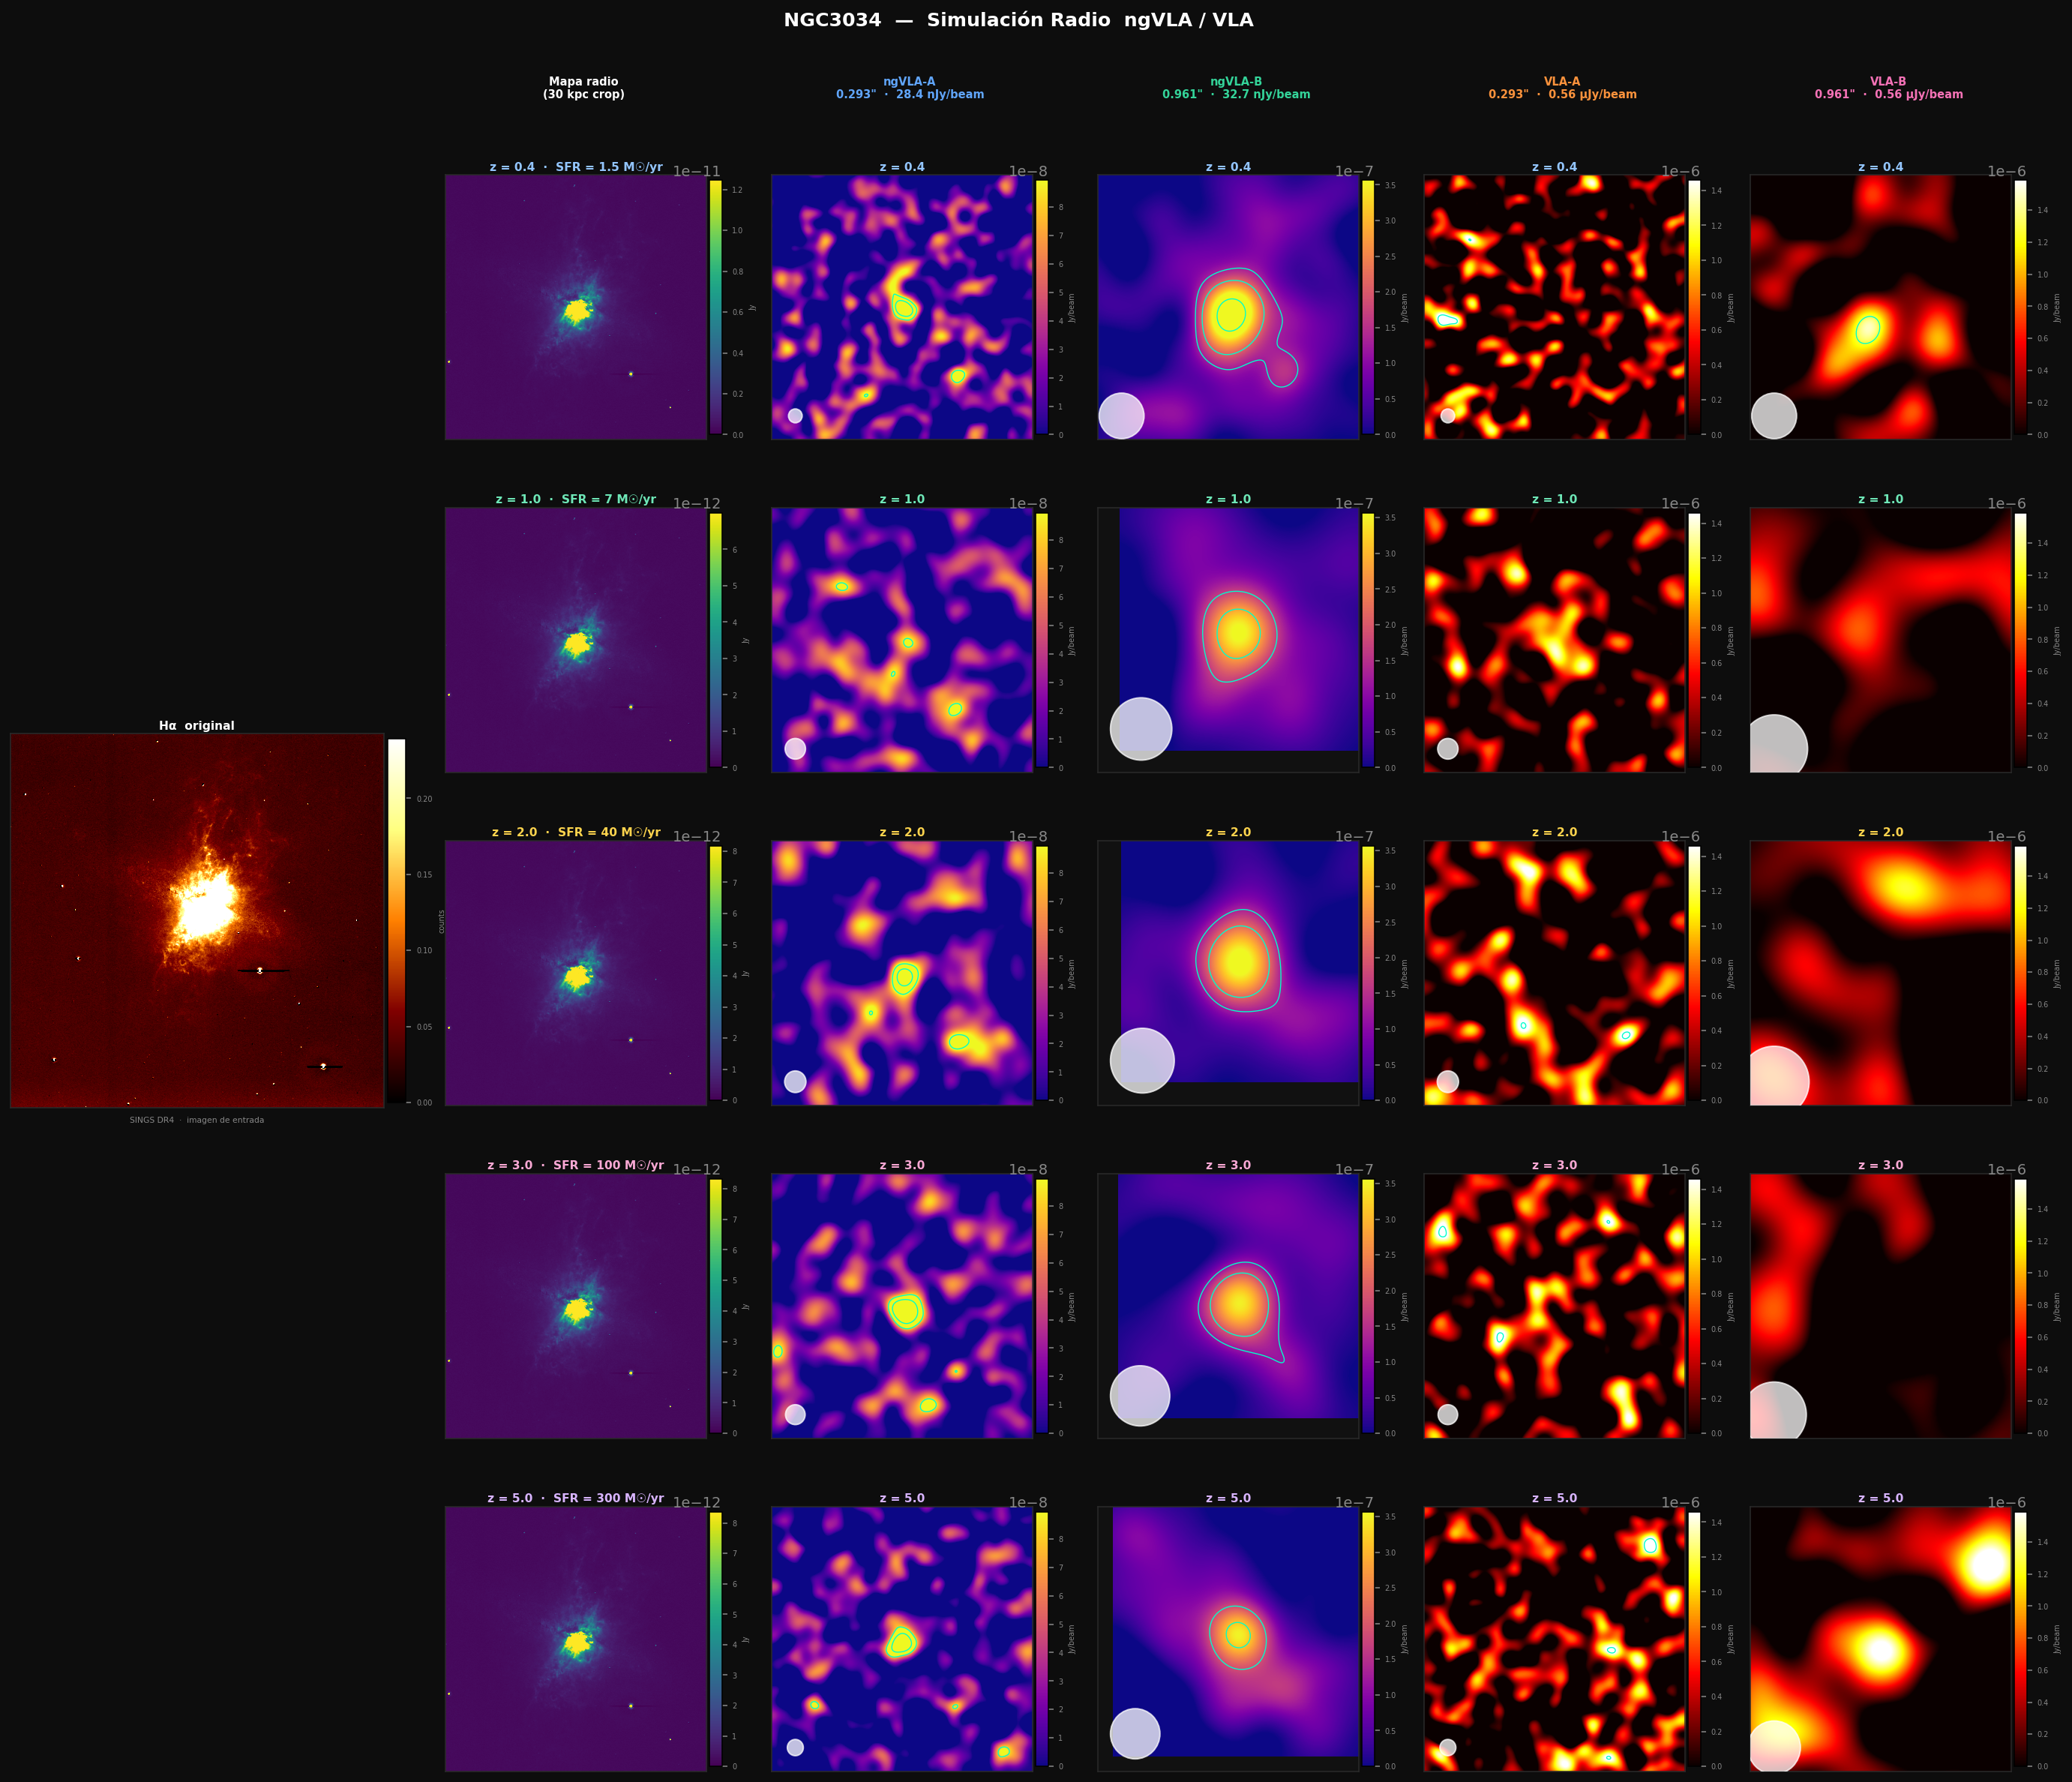
\includegraphics[height=0.72\textheight]{images/ngc3034.png}\\
    \footnotesize Núcleo compacto y brillante: 66.3\% del flujo H$\alpha$
    retenido sin ajustes; resuelto muy por encima de 3$\sigma$ en las
    cuatro configuraciones y los cinco $z$ -- incluso en ngVLA-A.
\end{frame}

\begin{frame}{Caso 2 -- NGC 1097: validación del recorte centrado}
    \centering
    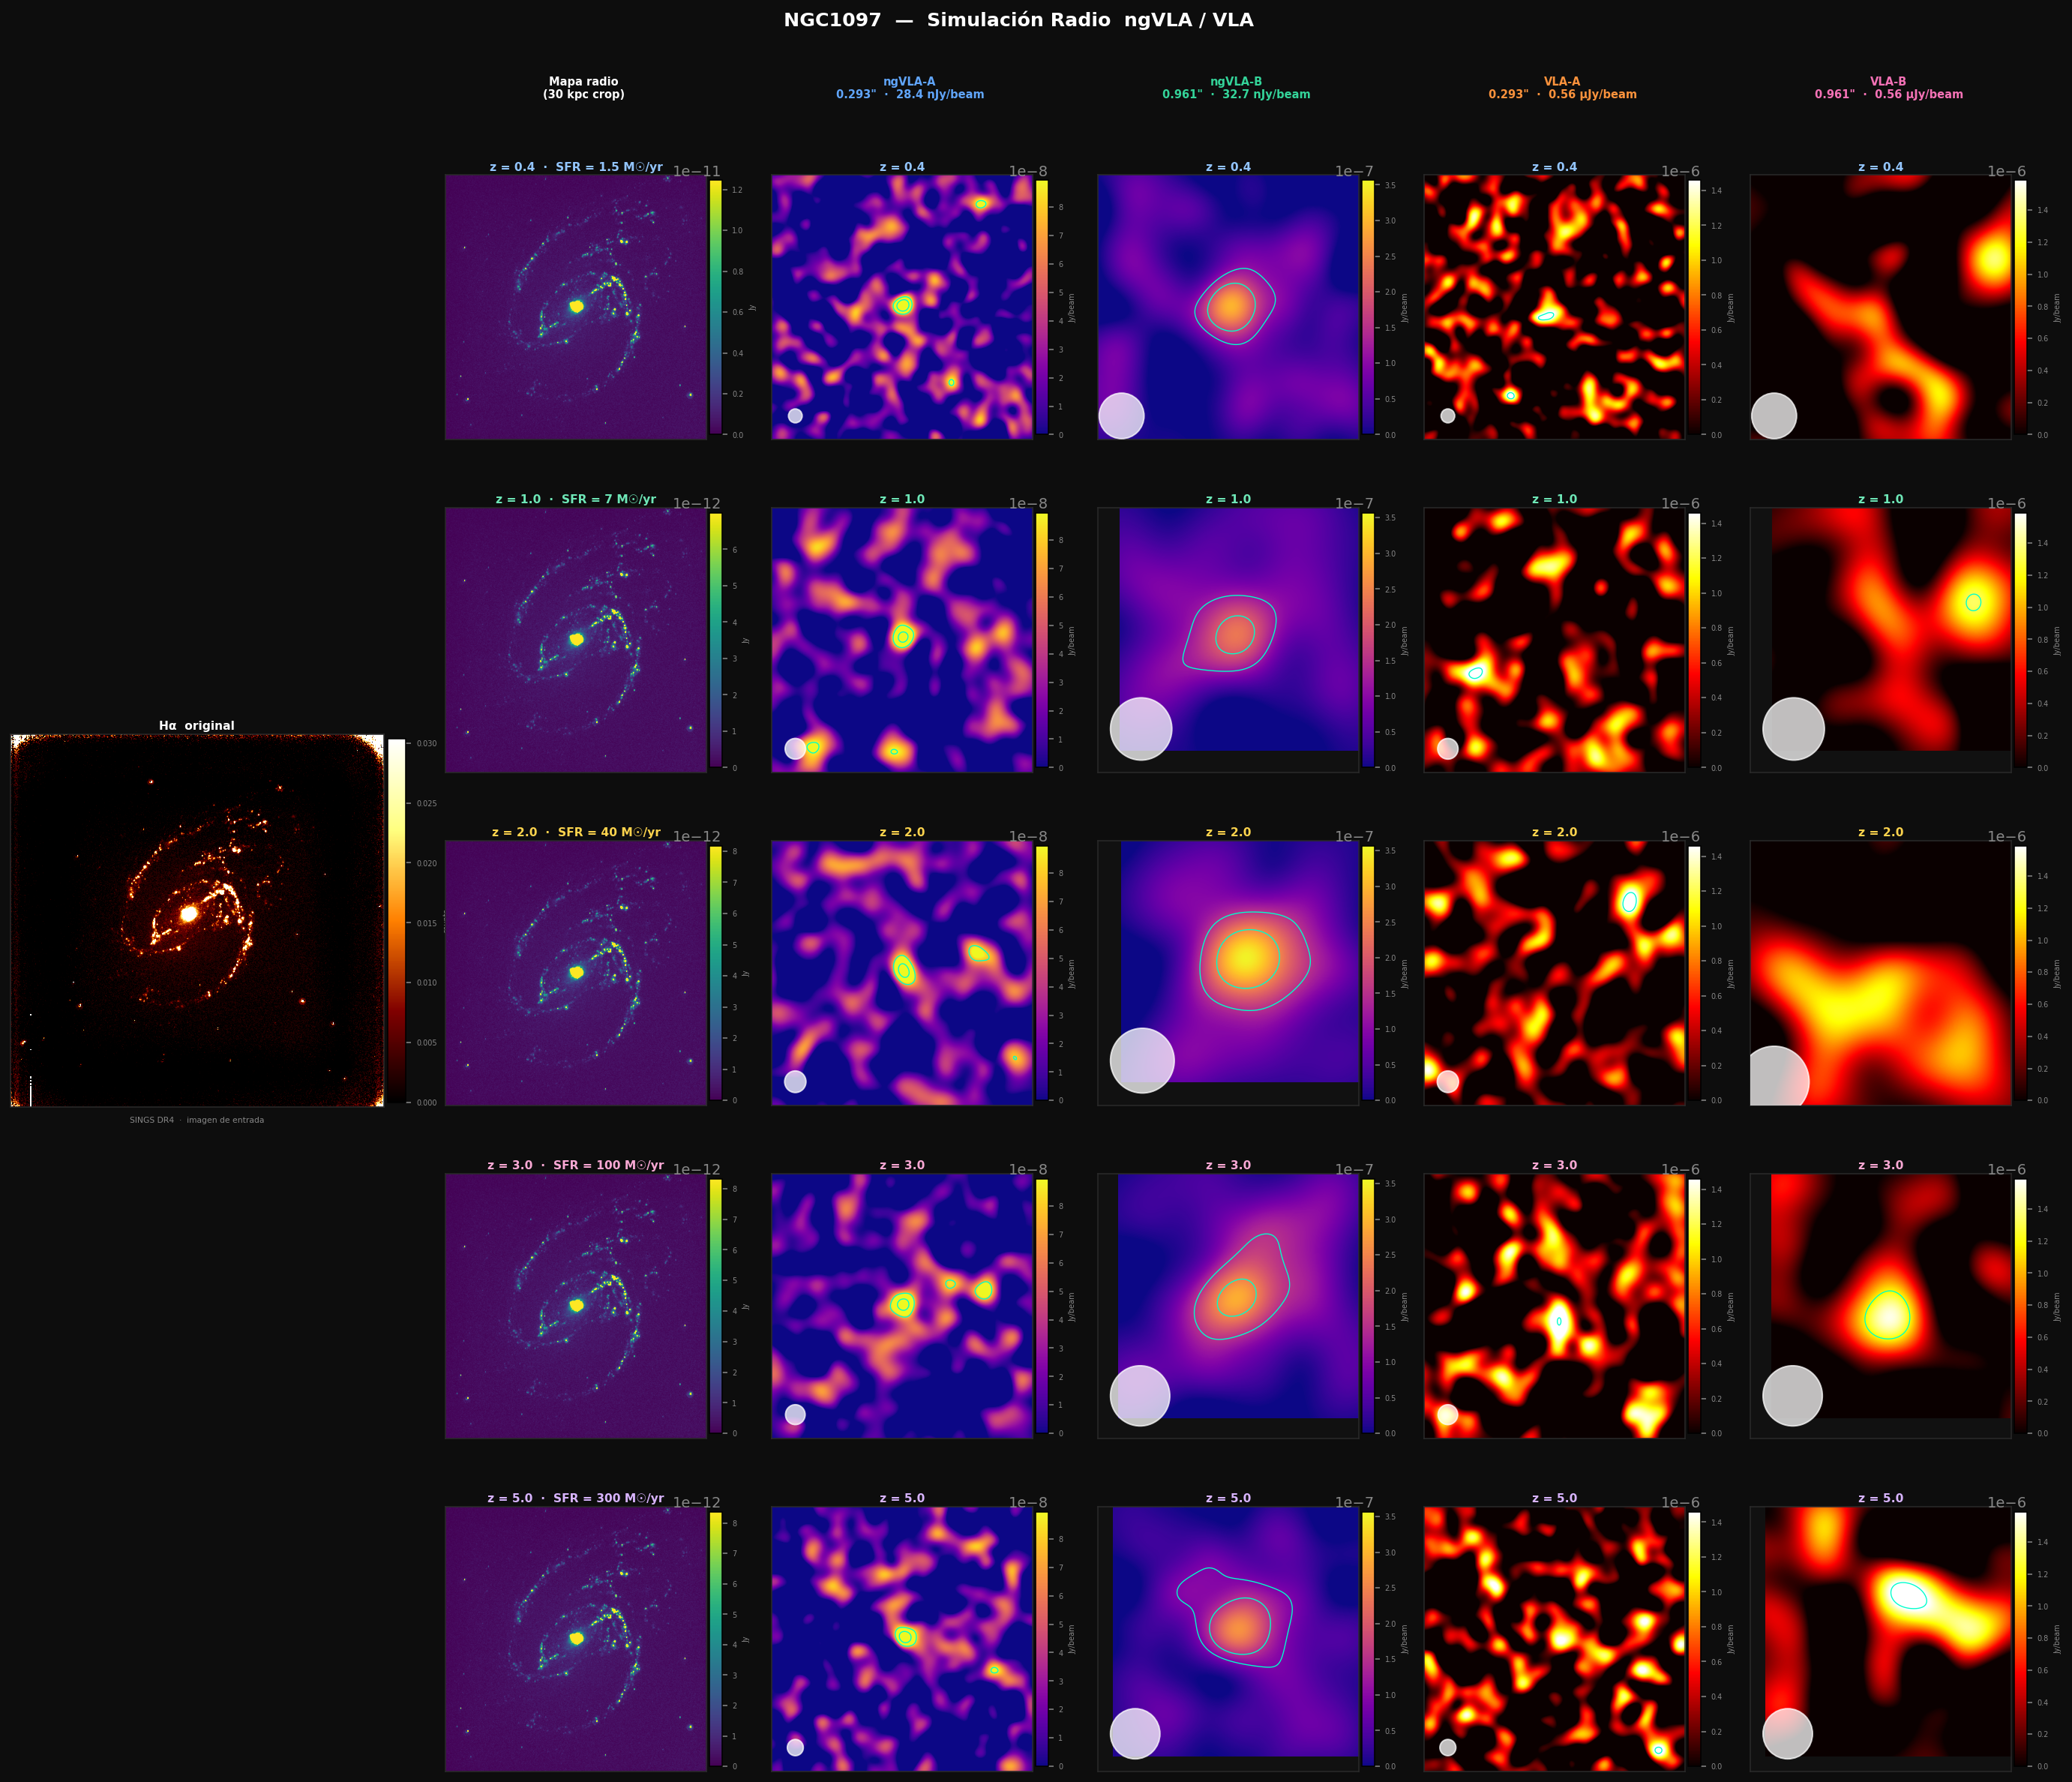
\includegraphics[height=0.72\textheight]{images/ngc1097.png}\\
    \footnotesize Antes del fix: solo 47.6\% del flujo dentro del recorte,
    emisión desplazada a una esquina. Tras el fix: anillo circumnuclear
    correctamente centrado en los cinco $z$.
\end{frame}

\begin{frame}{Caso 3 -- NGC 4254: validación de flujo positivo}
    \centering
    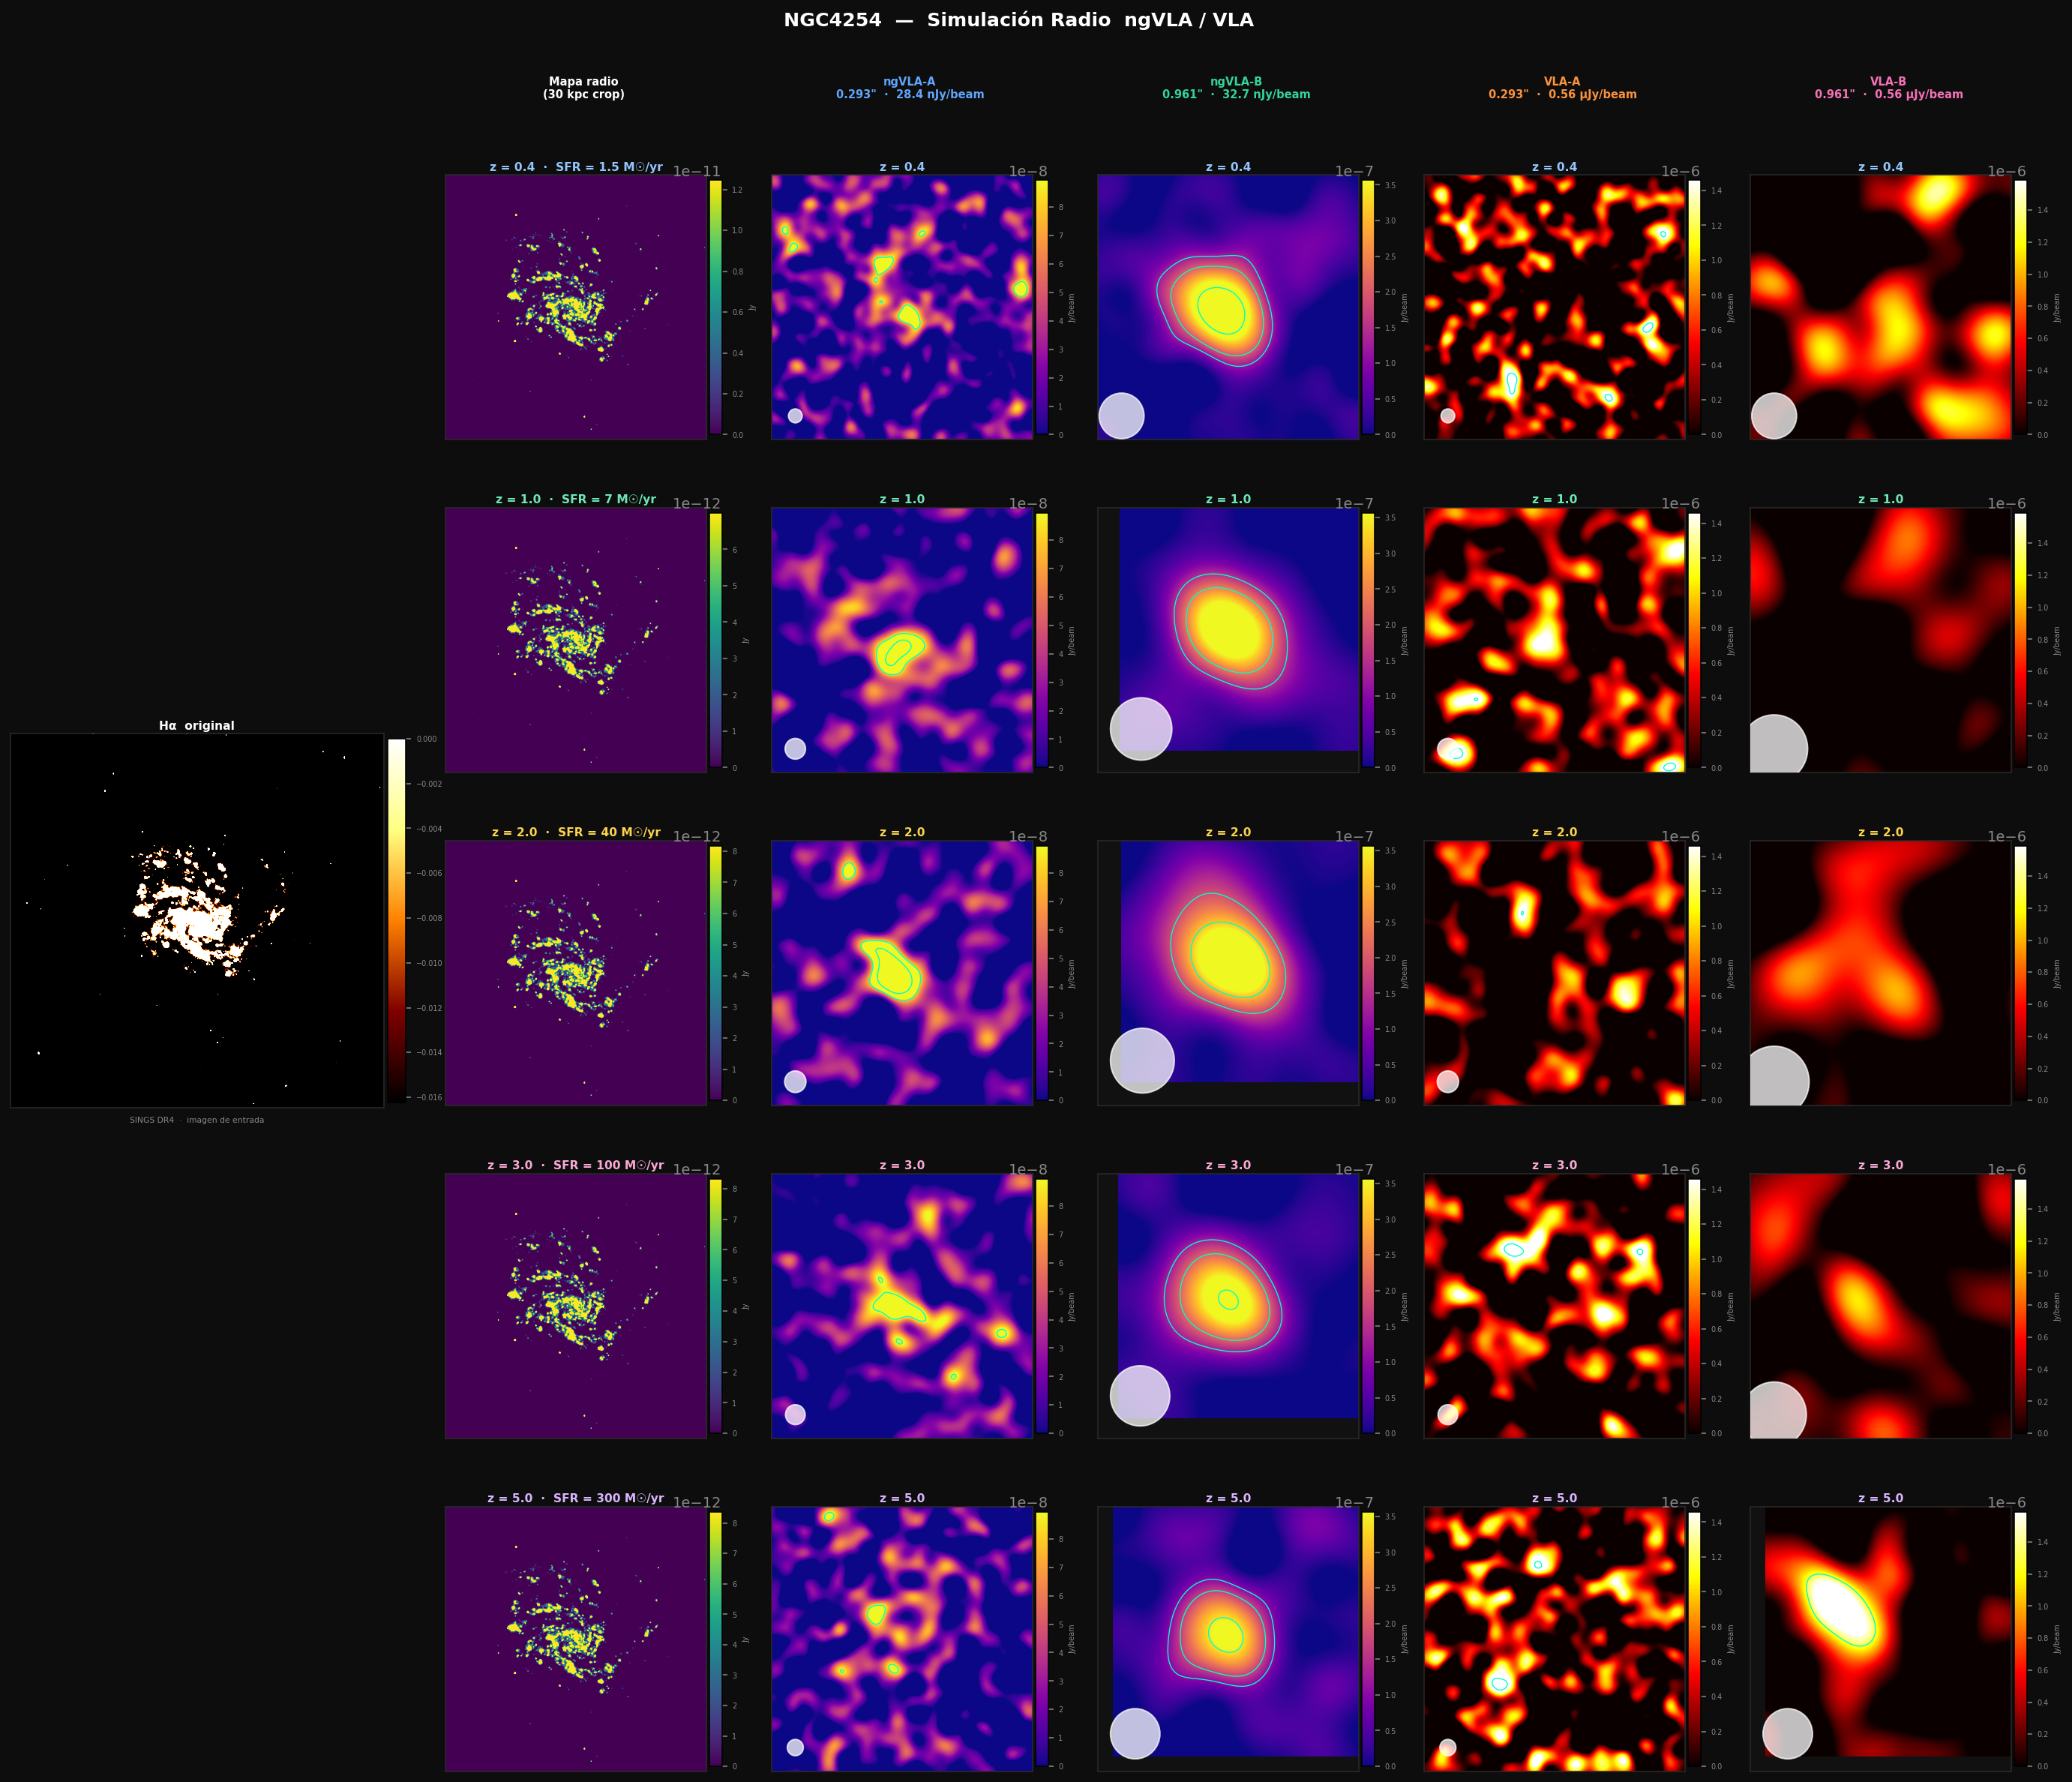
\includegraphics[height=0.72\textheight]{images/ngc4254_10ghz.png}\\
    \footnotesize 97.4\% de píxeles negativos invertía el signo del mapa
    de SFR. Tras el fix: disco floculento extendido recuperado; ngVLA-B
    traza contornos notablemente más extendidos que ngVLA-A (compromiso
    resolución-sensibilidad en su forma más clara de los tres casos).
\end{frame}

\begin{frame}{Complemento: banda L (1.4 GHz) vs.\ banda ngVLA (10 GHz)}
    \begin{itemize}
        \item Motivación: $S_\nu\propto\nu^{-\alpha}$ favorece más flujo
        a baja frecuencia, pero $\theta\sim\lambda/D$ empeora la
        resolución -- ¿cuál domina, para esta muestra?
        \item \texttt{SINGS\_1\_4GHz/}: mismo pipeline, beams/ruido
        recalculados a 1.4~GHz. VLA-B excluida (beam $6.864''$ supera el
        FOV recortado; \texttt{imsmooth} no converge).
    \end{itemize}
    \begin{center}
    \small
    \begin{tabular}{lccc}
    \toprule
    Config. & Beam & Ruido rms/beam & Subarreglo \\
    \midrule
    ngVLA-A & $0.99''$ & 62.41 nJy & Mid+Spiral+OuterCore \\
    ngVLA-B & $1.24''$ & 45.75 nJy & Main \\
    VLA-A   & $2.093''$ & 1.99 $\mu$Jy & -- \\
    \bottomrule
    \end{tabular}
    \end{center}
    \small Beams sustancialmente más anchos que a 10~GHz (peor
    resolución a menor frecuencia) -- comparación no perfectamente
    controlada (beams no emparejados entre instrumentos).
\end{frame}

\begin{frame}{Banda L: mejora sustancial de detectabilidad en ngVLA-A}
    \begin{center}
    \small
    \begin{tabular}{lccc}
    \toprule
    Galaxia & S/N, 10 GHz & S/N, 1.4 GHz & Métrica \\
    \midrule
    NGC 4254 & 4.0 -- 4.5 & 12 -- 21 & mediana / pico \\
    NGC 1097 & 3.4 -- 6.5 & 7.4 -- 14.2 & pico \\
    \bottomrule
    \end{tabular}
    \end{center}
    \centering
    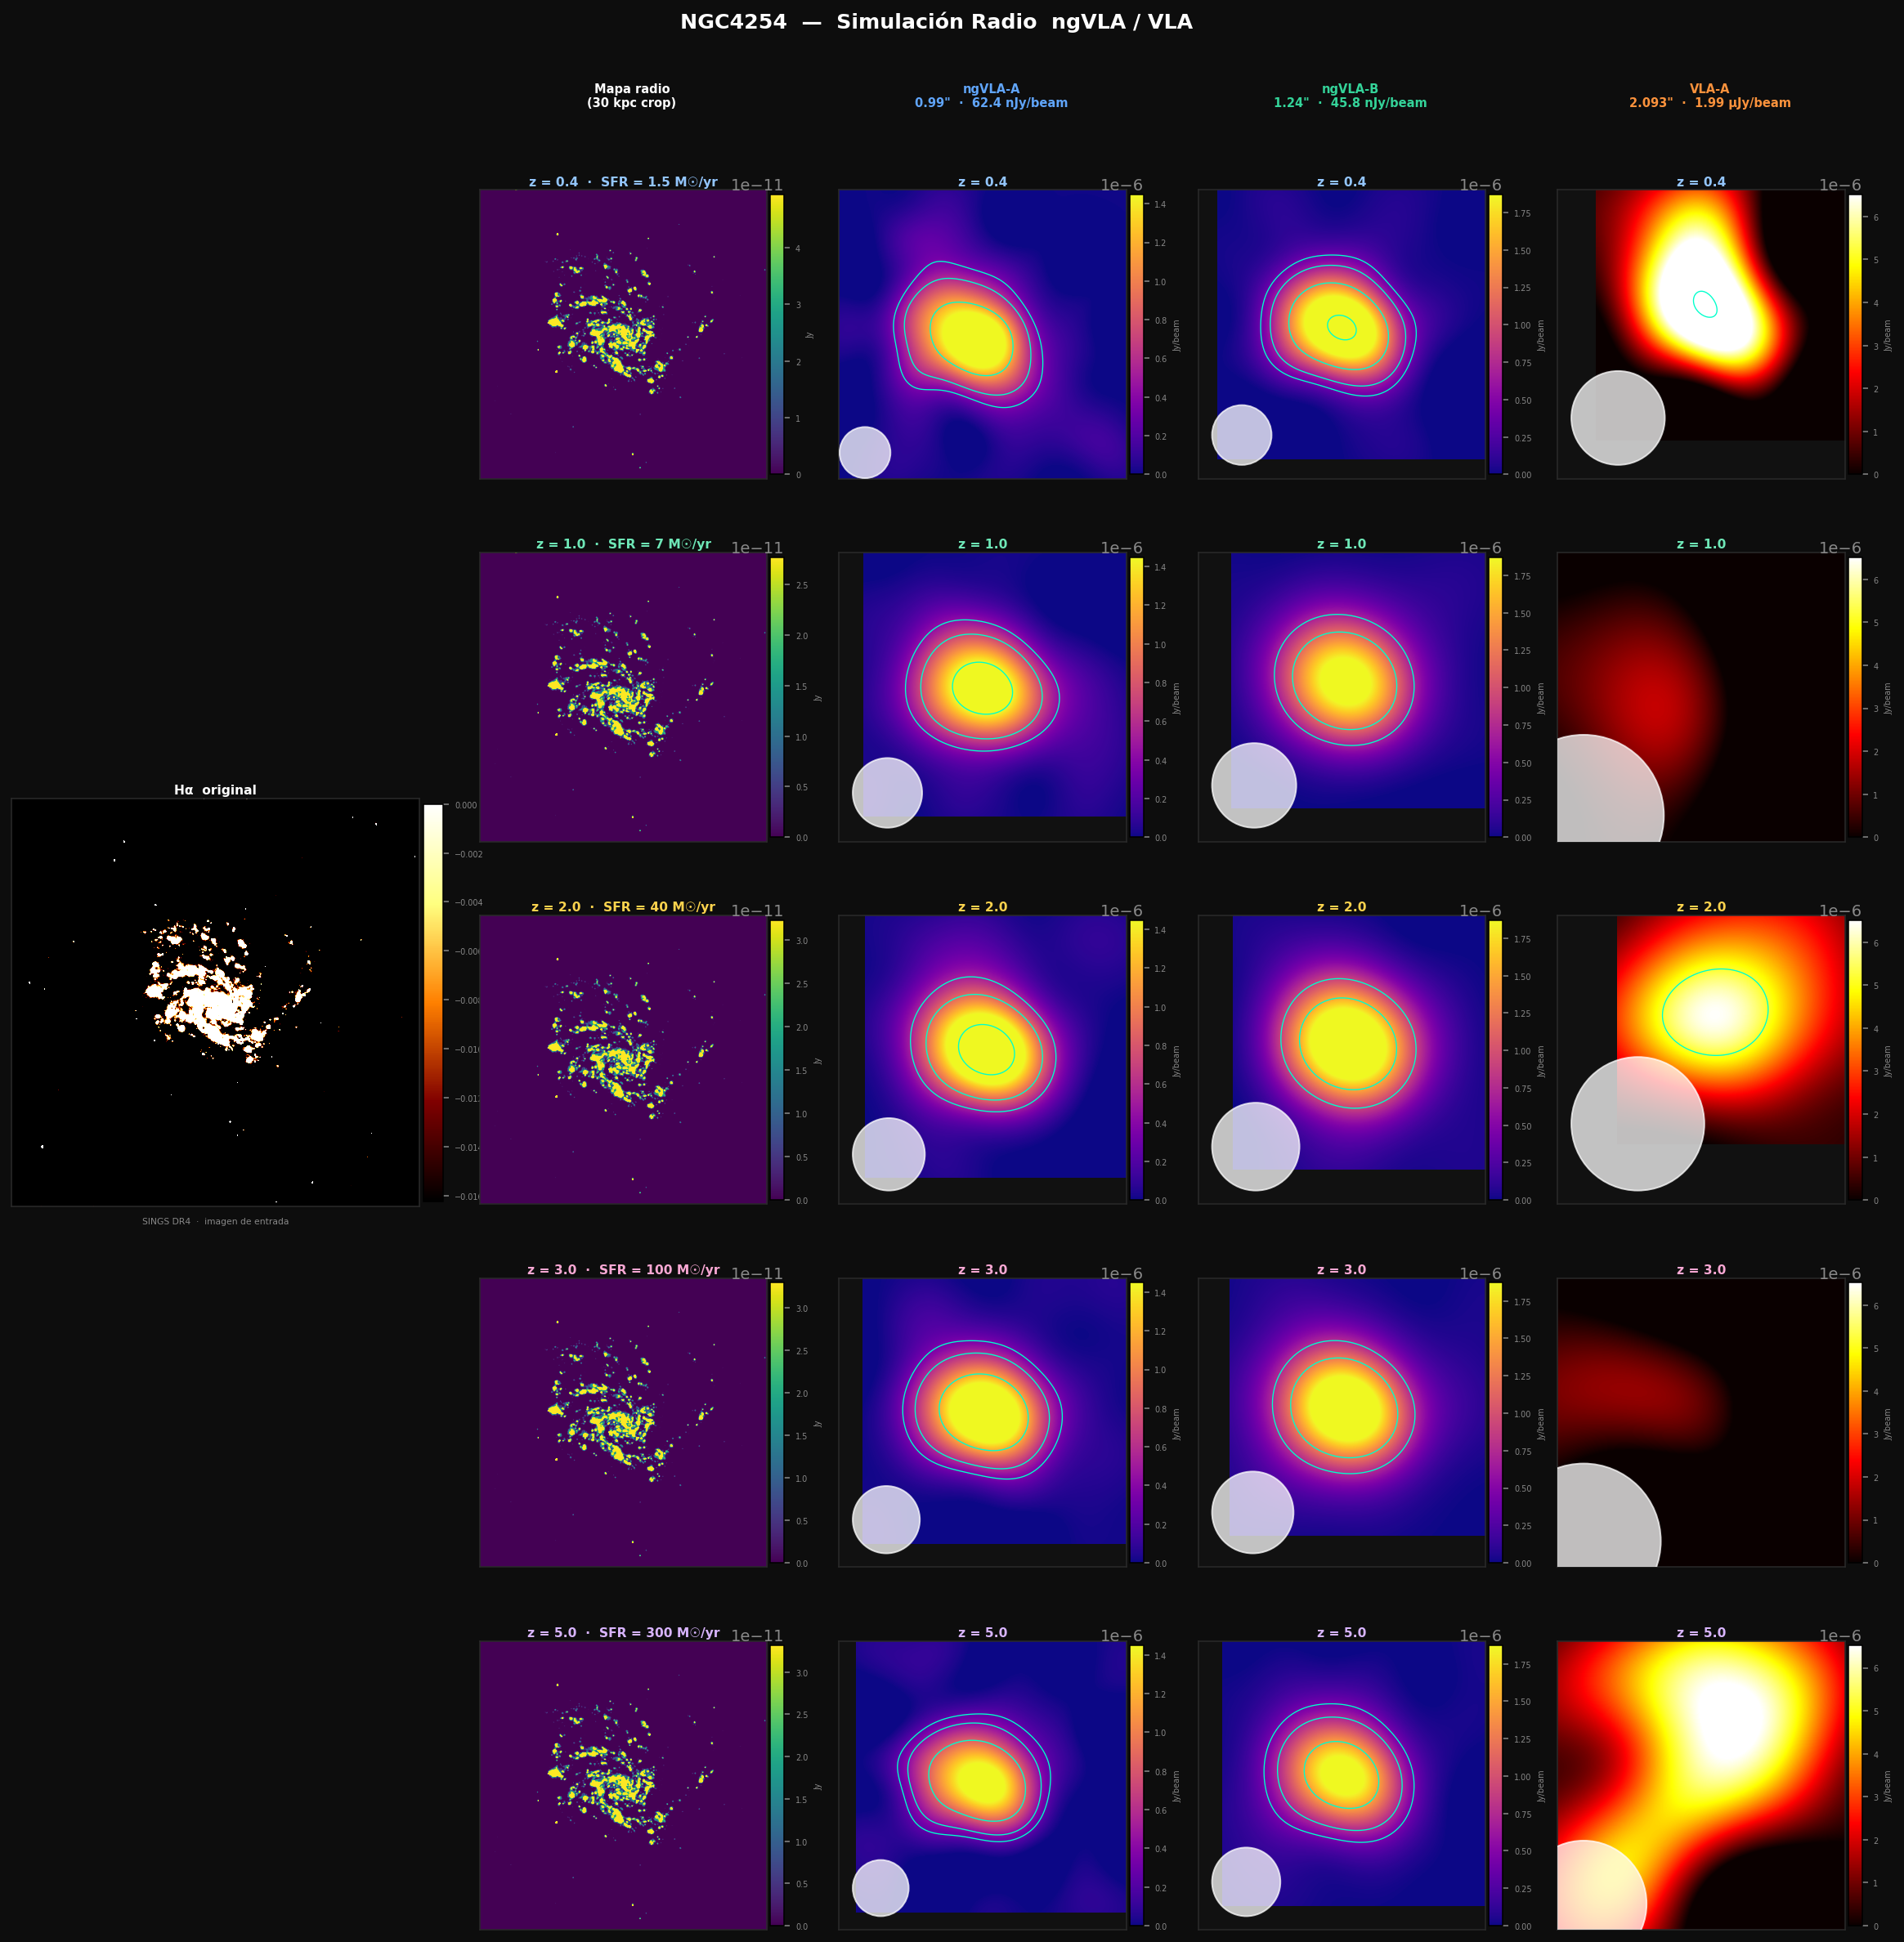
\includegraphics[height=0.55\textheight]{images/ngc4254_1_4ghz.png}\\
    \footnotesize NGC 4254 a 1.4 GHz: contornos claros hasta 20$\sigma$,
    vs.\ detección marginal/inconsistente a 10 GHz en ngVLA-A.
\end{frame}

% =================================================================
\section{Discusión}
% =================================================================

\begin{frame}{Interpretación}
    \begin{itemize}
        \item Los 3 casos representativos, tras las correcciones de
        control de calidad, muestran el comportamiento físico esperado
        $\Rightarrow$ las simulaciones no son artefactos numéricos.
        \item El rms medido consistente con el nominal (ngECT/ECT) valida
        el modelo de ruido: representación \emph{cuantitativa}, no solo
        cualitativa, de la sensibilidad instrumental.
        \item El compromiso A vs.\ B escala con cuánto se extiende la
        fuente (mínimo en M82, máximo en NGC~4254) $\Rightarrow$ la
        configuración óptima del ngVLA depende de la morfología esperada
        de la fuente.
        \item Banda L vs.\ banda ngVLA: mismo comportamiento por
        morfología en un régimen de ruido/resolución distinto (segunda
        validación cruzada, independiente del sigma-clipping); pero el
        VLA sigue indetectable en \emph{ambas} bandas $\Rightarrow$ la
        ventaja del ngVLA es de sensibilidad fundamental, no de estrategia
        de banda.
    \end{itemize}
\end{frame}

\begin{frame}{Limitaciones principales}
    \small
    \begin{columns}[T]
        \begin{column}{0.5\textwidth}
            \textbf{Física del modelo}
            \begin{itemize}
                \item Calibración radio--SFR y $\alpha$ únicos y fijos.
                \item H$\alpha$ sin corrección de extinción variable.
                \item Sin evolución morfológica/metalicidad con $z$.
                \item Cosmología y $M_*$ de referencia fijas.
            \end{itemize}
        \end{column}
        \begin{column}{0.5\textwidth}
            \textbf{Simulación instrumental}
            \begin{itemize}
                \item Beam gaussiano idealizado, no síntesis de plano $uv$
                completa (sin \texttt{simobserve}/\texttt{tclean}).
                \item Tiempo de integración fijo (20\,h).
                \item Ruido gaussiano estacionario (sin atenuación de
                \emph{primary beam}, RFI, etc.).
                \item S/N pico = 1 píxel; \texttt{crop\_size} no verificado
                en kpc reales por galaxia.
            \end{itemize}
        \end{column}
    \end{columns}
    \vfill
    \textbf{Cobertura}: 14/52 galaxias SINGS (por disponibilidad de
    H$\alpha$, no muestreo estadístico) -- no representativo del catálogo
    completo, sí demostración de viabilidad metodológica.
\end{frame}

% =================================================================
\section{Conclusiones}
% =================================================================

\begin{frame}{Síntesis final}
    \begin{alertblock}{Resultado central}
        A igual resolución angular y bajo el mismo tiempo de integración,
        el ngVLA ofrece $\sim$19--20$\times$ menos ruido rms que el VLA
        actual -- lo que, de sostenerse frente a una síntesis de apertura
        completa, extendería la detectabilidad de formación estelar en
        radio continuo hacia el \emph{cosmic noon} ($z\sim1$--3).
    \end{alertblock}
    \begin{itemize}
        \item Los 5 objetivos específicos se cumplieron: caracterización
        técnica del ngVLA, generación de mapas de entrada verificados,
        simulación instrumental completa, comparación sistemática de
        sensibilidad/resolución, y documentación de resultados.
        \item El experimento complementario en banda L confirma que la
        ventaja del ngVLA es de sensibilidad fundamental, reproducible
        bajo un régimen instrumental distinto.
    \end{itemize}
\end{frame}

\begin{frame}{Líneas de trabajo futuro}
    \begin{itemize}
        \item Simulación de síntesis de apertura completa (cobertura real
        del plano $uv$, en vez de convolución de beam idealizada).
        \item Extender la muestra más allá de las 14 galaxias con
        H$\alpha$ disponible.
        \item Completar banda L: incorporar VLA-B y el subarreglo Core
        del ngVLA (requiere ajustar \texttt{crop\_size} en función del
        beam).
        \item Explorar el efecto de variar el tiempo de integración
        (fijo en 20\,h en este trabajo).
        \item Incorporar ALMA y un trazador de gas molecular, para el
        estudio conjunto de formación estelar y contenido de gas a alto
        $z$.
    \end{itemize}
\end{frame}

\begin{frame}
    \centering
    \Large \textbf{Gracias}\\[0.3cm]
    \normalsize Preguntas y comentarios\\[1cm]
    \small Código completo:
    \url{https://github.com/LobsangM/ngVLA_Research_Program}
\end{frame}

% ---------------------------------------------------------------
\begin{frame}[allowframebreaks]{Referencias}
    \tiny
    \bibliographystyle{plainnat}
    \bibliography{../informe/referencias}
\end{frame}

\end{document}
